\chapter{}\label{chap7}

\begin{enumerate}
\renewcommand{\labelenumi}{\bf\theenumi.}
\itemsep=5pt

\item 3 ಏಳು ಬಳಸಿ 20 ಬರಿಸಿ. ದಶಮಾಂಶವನ್ನೊಳಗೊಂಡಂತೆ ಯಾವುದೇ ಗಣಿತ ಪ್ರಕ್ರಿಯೆ ಬಳಸಬಹುದು. 

\item 4 ಸಲ 9 ಬಳಸಿ 20 ಬರಿಸಿ. 

\item 1 ರಿಂದ 9 ರವರೆಗಿನ ಅಂಕಿಗಳನ್ನು ಒಮ್ಮೆ ಮಾತ್ರ ಬಳಸಿ $\dfrac{1}{2}$ ಬರಿಸಿ. ದಶಮಾಂಶ ಒಳಗೊಂಡಂತೆ ಯಾವುದೇ ಗಣಿತ ಪ್ರಕ್ರಿಯೆ ಬಳಸಬಹುದು. 

\item 1, 2, 3, 4, 5, 6, 7 ಇವು ಇದೇ ಕ್ರಮದಲ್ಲಿದ್ದು ನಡುವೆ ಯಾವುದೇ ಚಿಹ್ನೆ ಬಳಸಿ 100 ಬರಿಸಿ 

\item 1 ರಿಂದ 9ವರೆಗಿನ ಅಂಕಿಗಳನ್ನು ಒಮ್ಮೆ ಮಾತ್ರ ಬಳಸಿ 1 ಬರಿಸಿ. ಉತ್ತರ ಒಂದೇ ಸಂಖ್ಯೆಯಲ್ಲಿರಬೇಕು

\item ನಾಲ್ಕು 2 ಜೋಡಿಸಿ 5  ಬರಿಸಿ 

\item M ಬಾಹುಗಳನ್ನು ಪುನರ್ಜೋಡಿಸಿ, 1 ಬರಿಸಿ. 

\item CVI = X ಗೆರೆಗಳನ್ನು ಸ್ಥಾನ ಪಲ್ಲಟ ಮಾಡಿ, ಸಮೀಕರಣ ಸರಿದೂಗಿಸಿ. $\neq$ ಬರುವಂತಿಲ್ಲ. 

\item IV $+$ I = II ಒಂದು ಗೆರೆ ಸ್ಥಾನ ಪಲ್ಲಟಮಾಡಿ, ಸಮೀಕರಣ ಸರಿದೂಗಿಸಿ. $\neq$ ಬರುವಂತಿಲ್ಲ

\item I $-$ X = XLI ಒಂದು ಗೆರೆ ಸ್ಥಾನ ಪಲ್ಲಟ ಮಾಡಿ ಸಮೀಕರಣ ಸರಿದೂಗಿಸಿ $\neq$ ಬರುವಂತಿಲ್ಲ

\item 24 ಬೆಂಕಿಕಡ್ಡಿಗಳಿವೆ. ಕಡ್ಡಿ ಮುರಿಯಬಾರದು. ಒಂದು ಕಡ್ಡಿಯ ಮೇಲೆ ಇನ್ನೊಂದು ಕಡ್ಡಿ ಇರಿಸಬಹುದು. $\dfrac{1}{2}$ ಕಡ್ಡಿ ಚೌಕಗಳು ಭಾಗಶಃ ಕಡ್ಡಿ ಚೌಕಗಳು ಬರಬಹುದು. ಇದನ್ನು ಬರಿಸಿ. 
\begin{itemize}
\item[(a)] 16 ಚೌಕಗಳು ($\frac{1}{2}$ ಕಡ್ಡಿ ಬಾಹು)
\item[(b)] 27 ಚೌಕಗಳು ($\frac{1}{3}$ ಕಡ್ಡಿ ಬಾಹು)
\item[(c)] 50 ಚೌಕಗಳು ($\frac{1}{5}$ ಕಡ್ಡಿ ಬಾಹು)
\end{itemize}

\item 12 ಬೆಂಕಿಕಡ್ಡಿಗಳಿಂದ ಚೌಕ ರಚಿಸಿದೆ. 
\begin{figure}[H]
\centering
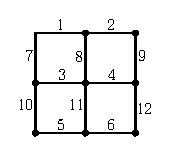
\includegraphics{images/chap7/q12.eps}
\end{figure}
\begin{itemize}
\item[(a)] 2 ಕಡ್ಡಿ ತೆಗೆದು 2 ಚೌಕ ಬರಿಸಿ ಅಳತೆ ಬೇರೆ ಬೇರೆ ಇರಬಹುದು 
\item[(b)] 4 ಕಡ್ಡಿ ತೆಗೆದು ಹಾಕಿ 2 ಸಮಾನ ಅಳತೆ ಚೌಕ ಬರಿಸಿ 
\item[(c)] 3 ಕಡ್ಡಿ ಸ್ಥಾನ ಪಲ್ಲಟ ಮಾಡಿ, 3 ಸಮಾನ ಅಳತೆ ಚೌಕ ಬರಿಸಿ 
\item[(d)] 4 ಕಡ್ಡಿ ಸ್ಥಾನ ಪಲ್ಲಟ ಮಾಡಿ 3 ಸಮಾನ ಅಳತೆ ಚೌಕ ಬರಿಸಿ 
\item[(e)] 2 ಕಡ್ಡಿ ಸ್ಥಾನ ಪಲ್ಲಟ ಮಾಡಿ, 7 ಚೌಕ ಬರಿಸಿ. ಅಳತೆ ಬೇರೆ ಬೇರೆ ಇರಬಹುದು 
\item[(f)] 4 ಕಡ್ಡಿ ಸ್ಥಾನ ಪಲ್ಲಟ ಮಾಡಿ 10 ಚೌಕ ಬರಿಸಿ . ಅಳತೆ ಬೇರೆ ಬೇರೆ ಇರಬಹುದು. 
\end{itemize}

\item ಈ ಗುಣಾಕಾರ ಗಮನಿಸಿ 

\begin{tabular}[t]{rcl}
$1\times 9 - 1$& = & $8$\\
$21\times 9 - 1$& = & $188$\\
$321\times 9 - 1$& = & $2888$\\
$4321\times 9 - 1$& = & $38888$\\
\end{tabular}

ಮುಂದಿನ 5 ಹಂತ ಬರೆಯಿರಿ. 

\item ಈ ಸಂಖ್ಯೆಗಳಲ್ಲಿ 9 ಇಲ್ಲ. ಅಂಕಿಗಳ ಪುನರಾವರ್ತನೆ ಇಲ್ಲ. ಅವನ್ನು 9 ರಿಂದ ಗುಣಿಸಿ. ಗುಣಲಬ್ಧ ನೋಡಿ. 1 ರಿಂದ 9 ವರೆಗೆ ಅಂಕಿಗಳಿವೆ.. ಪುನರಾವರ್ತನೆ ಇಲ್ಲ. 

\begin{tabular}[t]{lcl}
$58132764\times 9$ & = & $523194876$\\
$72645381\times 9$ & = & $653812479$\\
$76125483\times 9$ & = & $685129347$\\
$81274365\times 9$ & = & $731469285$
\end{tabular}

\item 17 ಸೇಬುಗಳಿವೆ. 4 ಸೇಬುಗಳ 8 ಸಾಲು, 5 ಸೇಬುಗಳ 2 ಸಾಲು ಬರುವಂತೆ ಜೋಡಿಸಿ. 

\item 4 ಏಕಕೇಂದ್ರೀಯ ವೃತ್ತಗಳಿವೆ. 4 ವ್ಯಾಸ ಎಳೆದಿದೆ. 8 ಬಿಂದುಗಳನ್ನು ಪ್ರತಿ ವ್ಯಾಸದ ಮೇಲೂ 2, ಪ್ರತಿ ವೃತ್ತ ಪರಿಧಿಯ ಮೇಲೂ 2 ಬರುವಂತೆ ಗುರ್ತಿಸಿ 

\item ಈ ಆಕೃತಿಯ ಎಲ್ಲ ಮನೆಗಳೊಳಗೂ ಚಲಿಸಬೇಕು. ಕಾಗದದಿಮ್ದ ಪೆನ್ಸಿಲ್ ಮೇಲೆತ್ತುವಂತಿಲ್ಲ. ಹಿಮ್ಮುಖ ಚಲನೆಯಿಲ್ಲ. ಒಂದು ರೇಖಾ ಖಂಡವನ್ನು ಒಮ್ಮೆ ಮಾತ್ರ ಕತ್ತರಿಸಬಹುದು. ಸರಳರೇಖೆ/ವಕ್ರ ರೇಖೆಯಾಗಬಹುದು. 

\begin{figure}[H]
\centering

\includegraphics{images/chap7/q17.eps}
\end{figure}

\item 9 ಒಂದೇ ಸಮನಾದ ರೇಖಾಖಂಡ ಬಳಸಿ, 5 ಸಮಬಾಹು ತ್ರಿಭುಜ ರಚಿಸಿ. 

\item ಸ್ವಾರ್ಧಂ ಪಾದಾ ಪ್ರಯಾಗೇ ನವಲನಯುಗಲಂ ಯೋವಶೇಷಾಚ್ಚ ಕಾಶ್ಯಾಂ 

ಶೇಷಾಂಘ್ರಿಂ ಶುಲ್ಕ ಹೋತೋಃ ಪಧಿದಶ ಮಯಾನ್ ಷಟ್ಟ ಶೇಷಾದ್ಗಯಾಯಾಂ 

ಶಿಷ್ಟಾ ನಿಷ್ಟ ತ್ರಿಶಷ್ಟಿರ್ನಿಜಗೃಹಮನಿಯಾ ತೀರ್ಥಪಾಂಧೀ ಪ್ರಯಾತ 

ತಸ್ಯದ್ರವ್ಯ ಪ್ರಮಾಣಂ ವದ ಯದಿ ಭವತಾ ಶೇಷಜಾತಿಃ ಶ್ರುತಾಸ್ತಿ ।।

\hfill (ಭಾಸ್ಕರಾಚಾರ್ಯರ `ಲೀಲಾವತೀ'ಯಿಂದ)


{\bf ಅರ್ಥ:} ಒಬ್ಬ ಯಾತ್ರಿಕನು ತನ್ನಲ್ಲಿದ್ದ ಹನದಲ್ಲಿ ಅರ್ಧಭಾಗವನ್ನು ಪ್ರಯಾಗದಲ್ಲಿಯೂ, ಉಳಿದುದರಲ್ಲಿ $\dfrac{2}{9}$ ಭಾಗವನ್ನು ಕಾಶಿಯಲ್ಲೂ, ಉಳಿದುದರಲ್ಲಿ $\dfrac{1}{4}$ ಭಾಗವನ್ನು ಮಾರ್ಗದಲ್ಲಿ ಸುಂಕಕ್ಕಾಗಿಯೂ, ಉಳಿದುದರಲ್ಲಿ $\dfrac{6}{10}$ ಭಾಗವನ್ನು ಗಯಾಕ್ಷೇತ್ರದಲ್ಲಿಯೂ ಖರ್ಚುಮಾಡಿ 6 ಕನಿಷ್ಟ (ಒಂದು ನಾಣ್ಯ)ಗಳೊಡನೆ ಮನೆಗೆ ಹಿಂದಿರುಗಿದನು. ಭಿನ್ನ ರಾಶಿಗಳ ವ್ಯತಕಲನ ಕ್ರಮವು ತಿಳಿದಿದ್ದಲ್ಲಿ, ಮೊದಲು ಅವನಲ್ಲಿದ್ದ ಹಣವೆಷ್ಟು ಹೇಳು.

\item ಪಂಚಾಂ ಶೋಲಿಕುಲಾ ತ್ಕದಂ ಮಗಮತ್ ತ್ರ್ಯಂಶಃ ಶಿಲೀಂಧ್ರಂತಯೋಃ 

ರ್ರಿ ಶ್ಲೇಷ ಸ್ತ್ರಿಗುಣೋ ಮೃಗಾಕ್ಷಿ ಕುಟಜಂ ದೋಲಾಯ ಮಾನೋತರಃ 

ಕಾಂತೇ ಕೇತಕ ಮಾಲತೀ ಪರಿಮಲ ಪ್ರಾಪ್ತೈಕ ಕಾಲತ್ರಿಯಾ ದೂತಾ ಹೂತ 

ಇತಸ್ತತೋಭ್ರಮತಿ ಖೇಭೃಂಗೋಲಿ ಸಂಖ್ಯಾಂವದ ।

ಅರ್ಥ: ಎಲೈಮೃಗಾಕ್ಷಿ ! ದುಂಬಿಗಳ ಒಂದು ಗುಂಪಿನಿಂದ $\dfrac{1}{5}$ ಭಾಗವು ಕದಂಬ ಪುಷ್ಪವನ್ನು, $\dfrac{1}{3}$ ಭಾಗವು ಶಿಲೀಂಧ್ರ ಪುಷ್ಪರನ್ನೂ, ಈ ಭಾಗಗಳ ಅಂತರದ 3ರಷ್ಟು ಕುಟಜ ಪುಷ್ಪವನ್ನು ಸೇರಿದುವು. ಮಿಕ್ಕ ಒಂದು ದುಂವಿಯು ಕೇತಕ ಮತ್ತು ಮಾಲತಿ ಎಂಬ ಎರುಡು ಪುಷ್ಪಗಳಿಂದಲೂ ಆಕರ್ಷಿತವಾಗಿ, ಅಂತರಿಕ್ಷದಲ್ಲಿ ಅಲ್ಲಿಂದಿಲ್ಲಿಗೆ ಹಾರಾಡುತ್ತಿದೆ. ಗುಂಪಿನಲ್ಲಿದ್ದ ದುಂಬಿಗಳೆಷ್ಟು?  

\item ಎರಡು 1ಗಳು (1, 1) ಮತ್ತು ಎರಡು 0ಗಳು (0, 0) ಬಳಸಿ ಮಾಡಬಹುದಾದ ಅತಿ ದೊಡ್ಡ ಸಂಖ್ಯೆ ಯಾವುದು? 

\item ನಿನ್ನಲ್ಲಿರುವ ಹಣ, ಅದರಷ್ಟೇ ಹಣ, ಅದರ 2ರಷ್ಟು ಹಣ, ಅದರ $\dfrac{1}{2}$ದಷ್ಟು ಹಣ - ಇವುಗಳ ಮೊತ್ತದಲ್ಲಿ 9ರೂ ಕಳೆದರೆ ನಿನ್ನಲ್ಲಿ ಏನೂ ಹಣ ಉಳಿಯುವುದಿಲ್ಲ. ನಿನ್ನಲ್ಲಿ ಮೊದಲಿದ್ದ ಹಣ ಎಷ್ಟು? 

\item ಎರಡಂಕಿ ಸಂಖ್ಯೆ ಬರೆಯಿರಿ. ಯಾರಿಗೂ ತೋರಿಸಬೇಡಿ. ಅಂಕಿಗಳ ವ್ಯತ್ಯಾಸ $> 1$ ಇರಬೇಕು. ಸಂಖ್ಯೆ ತಿರುವು ಮುರುವು ಮಾಡಿ. ದೊಡ್ಡದಲ್ಲಿ ಚಿಕ್ಕದು ಕಳೆಯಿರಿ. ಉತ್ತರದಲ್ಲಿನ ಒಂದು ಅಂಕ ಹೇಳಿ. ಇನ್ನೊಂದನ್ನು ನಾನು ಹೇಳುತ್ತೇನೆ. 

\item ಒಂದು ಸಂಖ್ಯೆ ಬರೆಯಿರಿ. 20ಕ್ಕಿಂತ ಹೆಚ್ಚಿರಲಿ ಅಂಕಿಗಳ ಮೊತ್ತ ಕಳೆಯಿರಿ. ಉತ್ತರದಲ್ಲಿ ಯಾವುದಾದರೂ 1 ಅಂಕಿ ಹೊಡೆದು ಹಾಕಿ. ಉಳಿದ ಅಂಕಗಳ ಮೊತ್ತ ಹೇಳಿ. ಹೊಡೆದು ಹಾಕಿದ ಅಂಕ ನಾನು ಹೇಳುತ್ತೇನೆ. 

\item 1 ಮೀಟರ್ ಬಾಹುವಿನ ಒಂದು ಮರದ ಘನ ಇದೆ. ಇದನ್ನು 1 ಸೆಂ.ಮೀ ಘನಗಳಾಗಿ  ಕತ್ತರಿಸಿ, ಸಣ್ಣ ಘನಗಳನ್ನು ಸಾಲಾಗಿ ಜೋಡಿಸಿದರೆ ಎಷ್ಟು ಉದ್ದ ಆಗುತ್ತದೆ. 

\item ಈ ಸಂಖ್ಯಾ ಸಮೀಕರಣಗಳನ್ನು ಗಮನಿಸಿ. ಅವು ಸರಿಯಾಗಬೇಕಂದರೆ ಸಂಖ್ಯೆಗಳ ನಡುವೆ ಒಂದು ಗಣಿತ ಪ್ರಕ್ರಿಯೆ ನಡೆಸಬೇಕು. ಆ ಪ್ರಕ್ರಿಯೆ ಪತ್ತೆ ಮಾಡಿ, `?' ಜಾಗದಲ್ಲಿರಬೇಕಾದ ಸಂಖ್ಯೆಯನ್ನು ಕಂಡು ಹಿಡಿಯಿರಿ (ಸ್ಪರ್ಧಾತ್ಮಕ ಪರೀಕ್ಷೆಯೊಂದರ ಸಮಸ್ಯೆ)

\begin{tabular}[t]{lcl}
$5-4$ & = & $23$\\
$8-1$ & = & $63$\\
$6-16$ & = & $32$\\
$9-9$ & = & $78$\\
$3-9$ & = & $6$\\
$3-81$ & = & $?$
\end{tabular}

\item ಈ ಸಂಖ್ಯಾ ವಿಚಿತ್ರ ಗಮನಿಸಿ. 

\begin{tabular}[t]{ccl}
$1552+5521+5215+2155$ & = & $14443$\\
$155+552+521+215$ & = & $1443$\\
$15+55+52+21$ & = & $143$\\
$1+5+5+2$ & = & $13$ 
\end{tabular}

ಮೊದಲ ಸಾಲಿನಲ್ಲಿ ಸಂಖ್ಯೆಯ ಮೊದಲ ಅಂಕಿ ಸ್ಥಾನ ಪಲ್ಲಟ ಮಾಡಿ ಕೊನೆಯ ಸ್ಥಾನದಲ್ಲಿ ಬರೆದಿದೆ. ಪ್ರಕ್ರಿಯೆ ಮುಂದುವರೆಸಿದೆ. 

2, 3, 4 ನೆ ಸಾಲುಗಳಲ್ಲಿ ಸಂಖ್ಯೆಯ ಕೊನೆಯ ಅಂಕಿ ಬಿಡಲಾಗಿದೆ. 

\item ಒಂದು ಬುಟ್ಟಿಯಲ್ಲಿ ಹಣ್ಣುಗಳಿವೆ. ಒಂದು ಸಲಕ್ಕೆ 2ರಂತೆ ತೆಗೆದರೆ 1 ಹಣ್ಣು ಉಳಿಯುತ್ತದೆ. ಒಂದು ಸಲಕ್ಕೆ 3, 4, 5, 6 ರಂತೆ ತೆಗೆದಾಗಲೂ 1 ಹಣ್ಣು ಉಳಿಯುತ್ತದೆ. ಒಂದು ಸಲಕ್ಕೆ 7ರಂತೆ ತೆಗೆದಾಗ ಹಣ್ಣು ಉಳಿಯುವುದಿಲ್ಲ. ಬುಟ್ಟಿಯಲ್ಲಿರ ಬಹುದಾದ ಕನಿಷ್ಠ ಸಂಖ್ಯೆಯ ಹಣ್ಣುಗಳೆಷ್ಟು? 

\item ಒಂದು ಸಂಖ್ಯೆ ಬರೆಯಿರಿ (5 ಅಥವಾ ಹೆಚ್ಚು ಅಂಕಿಗಳಿದ್ದರೆ ಉತ್ತಮ). ತಿರುವು ಮುರುವು ಮಾಡಿ ಬರೆಯಿರಿ. ಎರಡು ಸಂಖ್ಯೆಗಳನ್ನೂ ಬಲಗಡೆಯಿಂದ ಹೆಚ್ಚಿದ್ದರೆ ಮತ್ತೆ ಗುಂಪು ಮಾಡಿ. ಮೊತ್ತ ಬರೆಯಿರಿ. 

\begin{tabular}[t]{rr}
ಉದಾ: (1)\quad  $5,76,53,18$ & $8,13,56,75$\\
ಮೊತ್ತ\quad $1,52$ & $1,52$\\
$\underline{53}$ & $\underline{53}$\\
ಉದಾ: (2)\quad $92,36,47$  & $74,63,29$\\
$17,5$ & $1,66$\\
$76$ & $67$\\
ಅಂತಿಮ ಎರಡಂಕಿ ಸಮವಿರುತ್ತದೆ  & ಅಥವಾ ಒಂದರ ತಿರುವು ಮುರುವು ಇನ್ನೊಂದು 
\end{tabular}

\item ಯಾವುದೇ 2 ಸಂಖ್ಯೆ ಬರಿಯಿರಿ. ಗುಣಲಬ್ಧ ಬರೆಯಿರಿ. ಸಂಖ್ಯೆಗಳನ್ನು ತಿರುವು ಮುರುವು ಮಾಡಿ ಗುಣಿಸಿ. ಲಬ್ಧ ಪಡೆಯಿರಿ. ಎರಡು ಲಬ್ಧಗಳನ್ನು ಎರಡಂಕಿ ಗುಂಪು ಮಾಡಿ (ಬಲಗಡೆಯಿಂದ). ಗುಂಪುಗಳ ಮೊತ್ತ ಮಾಡಿ. ಅಂತಿಮ 2 ಅಂಕಿ ಬರುವವರೆಗೂ ಪ್ರಕ್ರಿಯೆ ಮುಂದುವರಿಸಿ. 

ಅಂತಿಮ ಉತ್ತರ ಒಂದೇ ಆಗಿರುತ್ತದೆ ಅಥವಾ ಒಂದರ ತಿರುವು ಮುರುವು ಇನ್ನೊಂದು ಆಗಿರುತ್ತದೆ. 

\begin{tabular}[t]{rr}
ಉದಾ: (1)\quad $427\times 689$ & $724\times 986$\\
$29,42,03$ & $71,38,64$\\
& $173$\\
$\underline{74}$ & $\underline{74}$\\
ಉದಾ: (1)\quad $817\times 956$ & $718\times 659$\\
$78,10,52$ & $47,31,62$\\
$1,40$ & $1,40$\\
$\underline{41}$ & $\underline{41}$
\end{tabular}
\end{enumerate}

\smallskip

\begin{center}
\rule{5cm}{1pt}\\[3pt]
{\Large\bfseries ಉತ್ತರಗಳು}\\[-0.1cm]
\rule{5cm}{1pt}
\end{center}

\begin{enumerate}
\item $\dfrac{7+7}{\cdot 7} = \dfrac{14}{\cdot 7} = \dfrac{140}{7} = 20$

\item $9 + \dfrac{99}{9} = 9 + 11 = 20$

\item $\dfrac{7\cdot 293}{14\cdot 586} = \dfrac{1}{2}$

\item $1+2+34+56+7 = 100$

\item $1^{23456789} = 1$

\item $2 + \dfrac{2}{2} + 2 = 5;\quad (2 \times 2)  + \dfrac{2}{2} = 5$

\item M \qquad VT = 1

\item $\sqrt{C} = X$

\item IV $-$ = III

\item L $-$ X = XL\quad \{XLI ನ 1ನ್ನು 1ಗೆ ಅಡ್ಡಲಾಗಿ ಬರೆದು L ಮಾಡಿದೆ\}

\item 1 ಬೆಂಕಿಕಡ್ಡಿ = 2 ಸೆಂ.ಮೀ ಇರಲಿ. 

\begin{itemize}
\item[(a)] 
\begin{figure}[H]
\centering
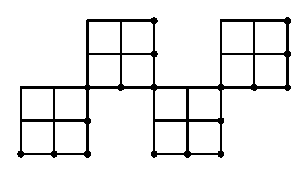
\includegraphics{images/chap7/ans11a.eps}
\end{figure}

ಪ್ರತಿ ಚೌಕದಲ್ಲಿಯೂ 6 ಬೆಂಕಿಕಡ್ಡಿ ಇದೆ. 

$\therefore\quad 6\times 4 = 24$ ಕಡ್ಡಿಗಳು 

ಒಟ್ಟು ಚೌಕಗಳು 24 ($\dfrac{1}{2}$ ಕಡ್ಡಿ)
\item[(b)]
\begin{figure}[H]
\centering
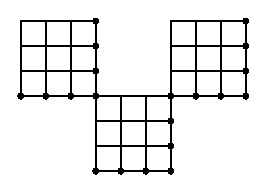
\includegraphics{images/chap7/ans11b.eps}
\end{figure}

ಪ್ರತಿ ಚೌಕದಲ್ಲಿಯೂ 8 ಬೆಂಕಿಕಡ್ಡಿಗಳಿವೆ. 

$\therefore\quad 3 \times 8 = 24$ಕಡ್ಡಿಗಳು 

ಪ್ರತಿ ಸಣ್ನ ಚೌಕವೂ $\dfrac{1}{3}$ ಕಡ್ಡಿ ಇದೆ. 

ಒಟ್ಟು ಚೌಕಗಳು $3 \times 9 = 27$
\item[(c)] 
\begin{figure}[H]
\centering
\includegraphics{images/chap7/ans11c.eps}
\end{figure}

ಪ್ರತಿ ದೊಡ್ಡ ಚೌಕವೂ 12 ಕಡ್ಡಿಗಳಿಂದ ಆಗಿದೆ. $12 \times 2 = 24$ ಕಡ್ಡಿಗಳು. ಪ್ರತಿ ದೊಡ್ಡ ಚೌಕದಲ್ಲಿಯೂ 25 ಚಿಕ್ಕ ಚೌಕಗಳಿವೆ. 

$25\times 2 = 50$ ಚೌಕಗಳು $\dfrac{1}{2}$ ಕಡ್ಡಿ ಅಳತೆ. 
\end{itemize}

\item 
\begin{itemize}
\item [(a)]
\begin{figure}[H]
\centering
\includegraphics{images/chap7/ans12a.eps}
\end{figure}

\item[(b)]
\begin{figure}[H]
\centering
\includegraphics{images/chap7/ans12b.eps}
\end{figure}

\item[(c)]
\begin{figure}[H]
\centering
\includegraphics{images/chap7/ans12c.eps}
\end{figure}

\item[(d)]
\begin{figure}[H]
\centering
\includegraphics{images/chap7/ans12d.eps}
\end{figure}


\item[(e)]
\begin{figure}[H]
\centering
\includegraphics{images/chap7/ans12e.eps}
\end{figure}

6, 12, ನ್ನು ಸ್ಥಾನ ಪಲ್ಲಟಮಾಡಿ ಒಮ್ದನ್ನು ಇನ್ನೊಂದು ಲಂಬವಾಗಿ ಕತ್ತರಿಸುವಂತೆ ಇರಿಸಿದೆ. 

\begin{tabular}{l}
4~ ಸಣ್ಣ ಚೌಕಗಳು ($\dfrac{1}{2}$ ಕಡ್ಡಿ ಅಳತೆ) \\
3~ ದೊಡ್ಡ ಚೌಕಗಳು (1 ಕಡ್ಡಿ ಅಳತೆ)\\
\hline
7~ ಚೌಕಗಳು\\
\hline
\end{tabular}

\item[(f)]
\begin{figure}[H]
\centering
\includegraphics{images/chap7/ans12f.eps}
\end{figure}

2, 9, 10, 5 ಇವುಗಳನ್ನು ಲಂಬವಾಗಿ ಕತ್ತರಿಸುವಂತೆ 2 ಚೌಕಗಳು ಅಳವಡಿಸಿದೆ. 

\begin{tabular}{lr}
ದೊಡ್ಡ ಚೌಕಗಳು & 2\\
ಚಿಕ್ಕ ಚೌಕಗಳು & 8\\
\hline
ಒಟ್ಟು & 10~ ಚೌಕಗಳು \\
\hline
\end{tabular}
\end{itemize}

\item 
\begin{tabular}[t]{ccl}
$33333\times 33335$ & = & $1111155555$\\
$333333\times 333335$ & = & $111111555555$\\
$3333333\times 3333335$ & = & $11111115555555$\\
$33333333\times 33333335$ &= & $1111111155555555$\\
$333333333\times 333333335$ & = & $111111111555555555$
\end{tabular}

\item ಉತ್ತರದ ಅಗತ್ಯವಿಲ್ಲ 

\item
\begin{figure}[H]
\centering
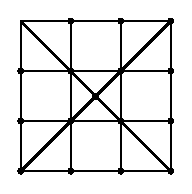
\includegraphics{images/chap7/ans15.eps}
\end{figure}

\begin{tabular}{ll}
4 ಅಡ್ಡ ಸಾಲುಗಳು & ಪ್ರತಿಯೊಂದರಲ್ಲಿಯೂ 4 ಸೇಬುಗಳು \\
4 ಕಂಭ ಸಾಲುಗಳು  & \\[0.2cm]
2 ಕರ್ಣಗಳು & 5 ಸೇಬುಗಳು 
\end{tabular}

\item
\begin{figure}[H]
\centering
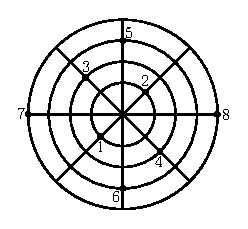
\includegraphics{images/chap7/ans16.eps}
\end{figure}


\item
\begin{figure}[H]
\centering
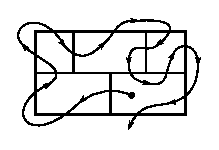
\includegraphics{images/chap7/ans17.eps}
\end{figure}

\item
\begin{figure}[H]
\centering
\includegraphics{images/chap7/ans18.eps}
\end{figure}

\begin{tabular}{l}
4 ಚಿಕ್ಕ ಸಮಬಾಹು ತ್ರಿಭುಜಗಳು\\
1 ದೊಡ್ಡ ಸಮಬಾಹು ತ್ರಿಭುಜಗಳು\\[0.2cm]
ಒಟ್ಟು 5 ಸಮಬಾಹು ತ್ರಿಭುಜಗಳು 
\end{tabular}

\item ಯಾತ್ರಿಕನಲ್ಲಿ ಪ್ರಾರಂಭಿಕ ಹಣ $x$ ನಿಷ್ಕ ಇರಲಿ 

ಪ್ರಯಾಗದಲ್ಲಿ $\dfrac{x}{2}$\qquad ಉಳಿಕೆ $\dfrac{x}{2}$
\begin{align*}
\text{ ಕಾಶಿ}\quad \dfrac{2}{9}\times \dfrac{x}{2} = \dfrac{x}{9}\quad;\quad \left(\dfrac{x}{2} - \dfrac{x}{9}\right) & = \dfrac{7x}{18}\\
\text{ ಸುಂಕ}\quad \dfrac{1}{4} \left(\dfrac{7x}{18}\right) = \dfrac{7x}{12} \quad;\quad \dfrac{7x}{18} - \dfrac{7x}{72} & = \dfrac{21x}{72} = \dfrac{7x}{24}\\
\text{ ಗಯಾ}\quad \dfrac{6}{10} \left(\dfrac{7x}{24}\right) = \dfrac{7x}{40}\quad;\quad \dfrac{7x}{24} - \dfrac{7x}{40} & = \dfrac{14x}{120}\\
\dfrac{14x}{120} = 63\quad;\quad 14x = 63\times 120 &\\
x = \dfrac{\cancel{63}^{9}\times \cancel{120}^{60}}{\cancel{14}_{7}} & = 540~\text{ ನಿಷ್ಕಗಳು}
\end{align*}

\item ದುಂಬಿಗಳ ಸಂಖ್ಯೆ $x$ ಇದಲಿ 
\begin{gather*}
\dfrac{x}{5} + \dfrac{x}{3} + 3 \left(\dfrac{x}{3} - \dfrac{x}{5}\right) + 1 = x\\
3x + 5x + 6x + 15 = 15x\\
15 - 14x = 15\\
x = 15\\
\therefore\quad 15 \text{ ದುಂಬಿಗಳು}
\end{gather*}


\item ಸಾಮಾನ್ಯವಾಗಿ ಎಲ್ಲರೂ ಹೇಳುವುದು 1100 ಆದರೆ ಈ ಸಂಖ್ಯೆ ಗಮನಿಸಿ $10^{10} = (1,000,000,0000)$ ಒಂದು ಸಾವಿದ ಕೋಟಿ. 

\item 
\begin{tabular}[t]{l}
ಮೊದಲಿನೆ ಹಣ $\rupee~ x$ ಇರಲಿ \\
ಅದರಷ್ಟೇ ಹಣ $\rupee~ x$  \\
ಅದರ 2ರಷ್ಟು ಹಣ $\rupee~ 2x$\\
ಅದರರ್ಧದಷ್ಟು ಹಣ $\rupee~ \dfrac{x}{2}$\\
\hline
ಒಟ್ಟು $\rupee~ 4\dfrac{1}{2}x$
\end{tabular}

ಇದರಲ್ಲಿ 9 ಕಳೆದರೆ $\rupee~ 4\dfrac{1}{2}x - 9 = 0$

$\dfrac{9x}{2} - 9 = 0\quad;\quad 9x - 18 = 0$

$\therefore 9x = 18\quad;\quad x = 2$

ಮೊದಲಿದ್ದ ಹಣ $\rupee~ 2$

\item ಇನ್ನೊಂದು ಅಂಕಿ 9ರ ಪೂರಕ 

ಉದಾ: ಸಂಖ್ಯೆ 84 ಇರಲಿ. ತಿರುವು ಮುರುವು 48 

$84 - 48 = 36$ ಇವು ಪರಸ್ಪರ 9ರ ಪೂರಕಗಳು 

\item ಹೊಡೆದು ಹಾಕಿದ ಅಂಕಿಯ ಮುಂದಿನ 9ರ ಗುಣಕದ ಪೂರಕ 

ಉದಾ: 45376 ಸಂಖ್ಯೆ ಇರಲಿ. ಅಂಕಿಗಳ ಮೊತ್ತ $4 + 5+ 3 + 7 + 6 = 25$

$45376 - 25 = 45\cancel{3}51$ 3ನ್ನು ಹೊಡೆದಿದೆ ಎಂದಿರಲಿ 

ಉಳಿದ ಅಂಕಿಗಳ ಮೊತ್ತ 15 ಮುಂದಿನ 9ರ ಗುಣಕ 18 

ಪೂರಕ 3 ಹೊಡೆದು ಹಾಕಿದ ಅಂಕಿ 

\item 1 ಮೀಟರ್ = 100 ಸೆಂ.ಮೀ

$\therefore\quad$ ಸಣ್ಣ ಘನಗಳ ಸಂಖ್ಯೆ $100\times 100\times 100 = 10,00,000$

ಒಂದು ಸಣ್ಣ ಘನ 1ಸೆಂ.ಮೀ. $\therefore\quad$ ಉದ್ದ $10,00,000$ ಸೆಂ.ಮೀ = $10,000$ ಮೀ = $10$ ಕಿ.ಮೀ 

\item 
\begin{tabular}[t]{lll}
& $5 - 4 = 23$ & $5^{2} - \sqrt{4} = 23$\\
& $8 - 1 = 63$ & $8^{2} - \sqrt{1} = 63$\\
& $6 - 16 = 32$ & $6^{2} - \sqrt{16} = 32$\\
& $9 - 9 = 78$ & $9^{2} - \sqrt{9} = 78$\\
& $3 - 9 = 6$ & $3^{2} - \sqrt{9} = 6$\\
$\therefore$ & $3 - 81 = ?$ & $3^{2} - \sqrt{81} = 0$
\end{tabular}

\item ಉತ್ತರದ ಅಗತ್ಯವಿಲ್ಲ 

\item 2, 3, 4, 5, 6 ರ ಲ.ಸಾ.ಅ. 60

$\therefore$ 60 $+$ 1 ಇದ್ದರೆ, 2, 3, 4, 5, 6 ರಂತೆ ತೆಗೆದಾಗ 1 ಹಣ್ಣು ಉಳಿಯುತ್ತದೆ. ಆದರೆ 7ರಂತೆ ತೆಗೆದಾಗ 5 ಉಳಿಯುತ್ತದೆ. 7ರಿಂದ ನಿಶ್ಶೇಷವಾಗಿ ಭಾಗವಾಗುವ ಸಂಖ್ಯೆ ಬೇಕು.

\begin{tabular}{ll}
$60\times 2 = 120 + 1$ & ಪರೀಕ್ಷಿಸಿ 7ರಿಂದ ನಿಶ್ಶೇಷವಾಗಿ ಭಾಗವಾಗುವುದಿಲ್ಲ\\
$60\times 3 = 180 + 1$ & ಪರೀಕ್ಷಿಸಿ 7ರಿಂದ ನಿಶ್ಶೇಷವಾಗಿ ಭಾಗವಾಗುವುದಿಲ್ಲ\\
$60\times 4 = 240 + 1$ & ಪರೀಕ್ಷಿಸಿ 7ರಿಂದ ನಿಶ್ಶೇಷವಾಗಿ ಭಾಗವಾಗುವುದಿಲ್ಲ\\
$60\times 5 = 300 + 1 = 301$ & ಇದು 7ರಿಂದ ನಿಶ್ಶೇಷವಾಗಿ ಭಾಗಿಸಲ್ಪಡುತ್ತದೆ. 
\end{tabular}

$\therefore\quad$ ಬುಟ್ಟಿಯಲ್ಲಿರಬಹುದಾದ ಕನಿಷ್ಠ ಸಂಖ್ಯೆ ಹಣ್ಣುಗಳು 301

\item ಉತ್ತರದ ಅಗತ್ಯವಿಲ್ಲ.

\item ಉತ್ತರದ ಅಗತ್ಯವಿಲ್ಲ .
\end{enumerate}
